\documentclass[border=4pt]{standalone}
\usepackage{amsmath,amssymb}
\usepackage{tikz}
\usetikzlibrary{arrows.meta,fit,backgrounds,calc}
\definecolor{cfg}{HTML}{2E7D46}
\definecolor{mcfb}{HTML}{2166AC}
\definecolor{negr}{HTML}{B03A2E}
\definecolor{inkc}{HTML}{1B1B1B}
\definecolor{gy}{HTML}{6B7280}
\definecolor{atg}{HTML}{6A4C93}
\begin{document}
\hyphenpenalty=10000\exhyphenpenalty=10000
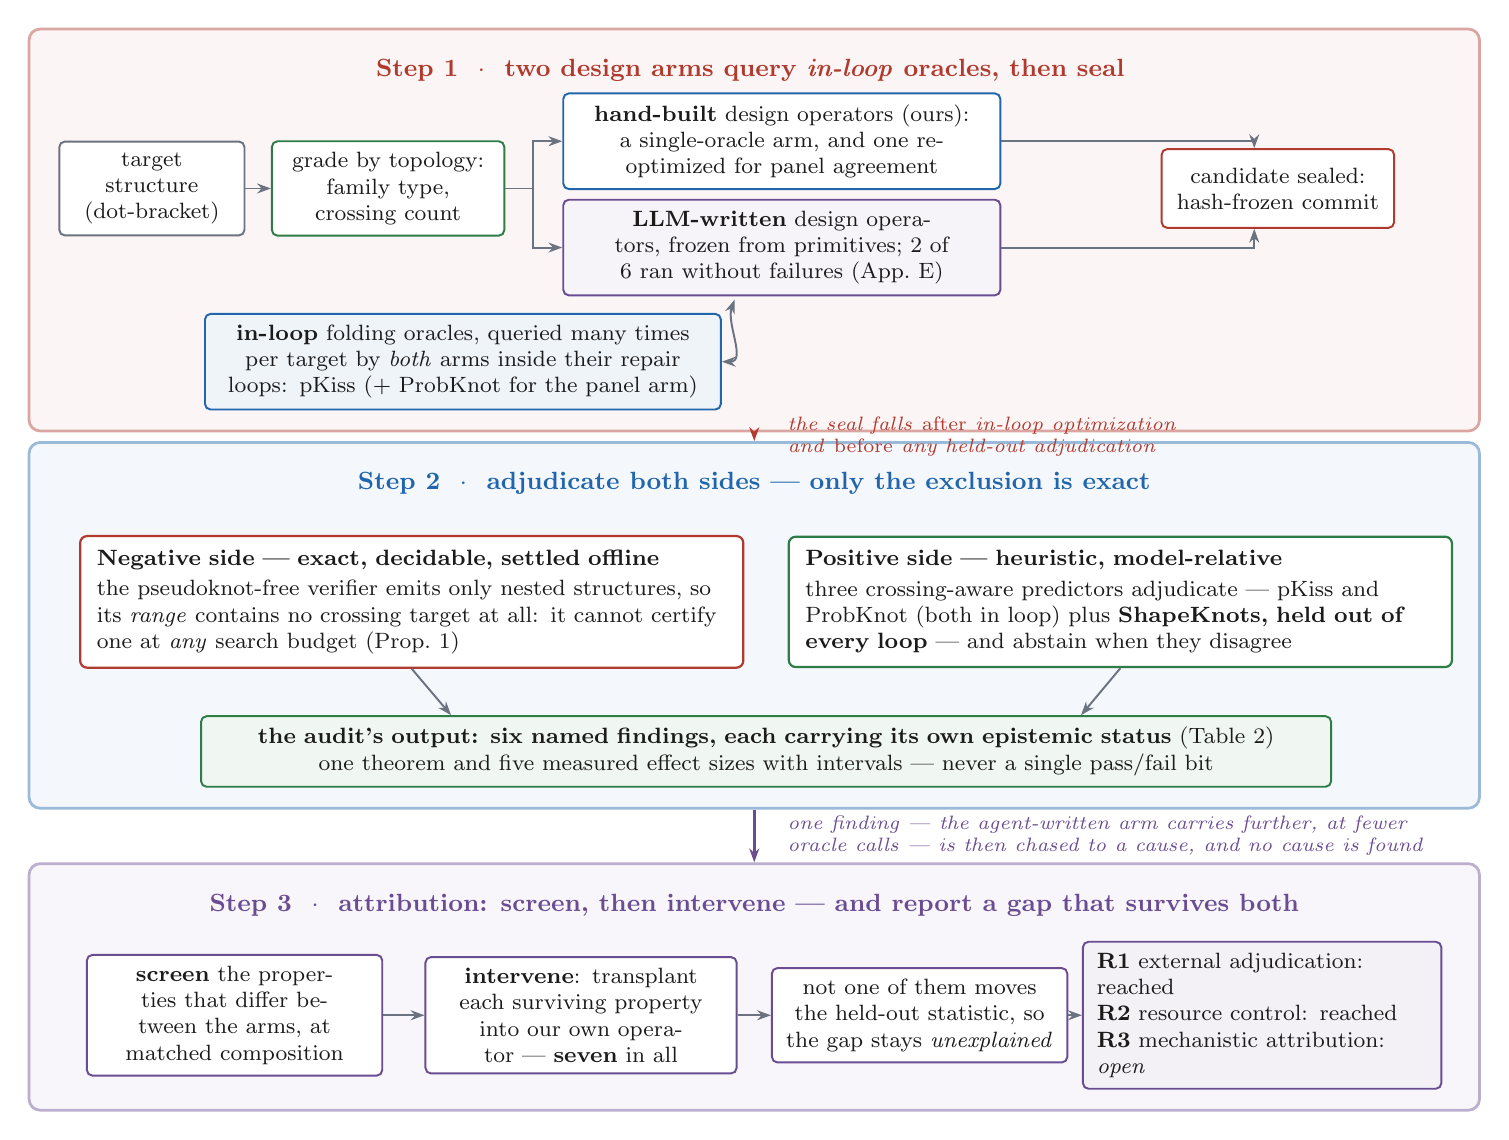
\begin{tikzpicture}[
  >={Stealth[length=5pt,width=3.6pt]},
  font=\footnotesize,
  bx/.style={draw=gy, line width=0.7pt, rounded corners=2pt, align=center, inner xsep=5pt, inner ysep=4pt,
             minimum height=10mm, fill=white, text=inkc},
  cf/.style={bx, draw=cfg}, mc/.style={bx, draw=mcfb}, ng/.style={bx, draw=negr}, ag/.style={bx, draw=atg},
  side/.style={draw, line width=0.8pt, rounded corners=2.5pt, align=left, inner xsep=6pt, inner ysep=5pt,
               fill=white, text=inkc, text width=80mm},
  reg/.style={rounded corners=4pt, line width=1pt, inner sep=2.6mm},
  rt/.style={font=\small\bfseries},
  df/.style={->, line width=0.7pt, draw=gy},
  cmt/.style={->, line width=0.9pt, draw=negr},
  ann/.style={font=\scriptsize\itshape, anchor=west, align=left},
]
% ==================== Step 1 : two design arms, in-loop oracles, sealed commit ====================
\node[bx, text width=20mm] (t) at (2.00,10.10) {target structure\\(dot-bracket)};
\node[cf, text width=26mm] (g) at (5.00,10.10) {grade by topology:\\family type,\\crossing count};
\node[mc, text width=52mm, minimum height=8mm] (armA) at (10.00,10.70)
  {\textbf{hand-built} design operators (ours): a single-oracle arm, and one re-optimized for panel agreement};
\node[ag, text width=52mm, minimum height=8mm, fill=atg!6] (armB) at (10.00,9.35)
  {\textbf{LLM-written} design operators, frozen from primitives; $2$ of $6$ ran without failures (App.~E)};
\node[ng, text width=26mm] (s) at (16.30,10.10) {candidate sealed:\\hash-frozen commit};
\draw[df] (t.east)--(g.west);
\draw[df] (g.east) -- ++(0.35,0) |- (armA.west);
\draw[df] (g.east) -- ++(0.35,0) |- (armB.west);
\draw[df] (armA.east) -| ([xshift=-3mm]s.north);
\draw[df] (armB.east) -| ([xshift=-3mm]s.south);
\begin{scope}[on background layer]
  \node[fit=(armA)(armB), inner sep=1pt] (arms) {};
\end{scope}
\node[mc, text width=62mm, minimum height=7mm, fill=mcfb!7] (inl) at (5.95,7.90)
  {\textbf{in-loop} folding oracles, queried many times per target by \emph{both} arms inside their
   repair loops: pKiss ($+$ ProbKnot for the panel arm)};
\draw[df, <->] (inl.east) to[out=0,in=250] ([xshift=-6mm]arms.south);
\node[rt, text=negr] (st1) at (9.60,11.60) {Step 1\ \ $\cdot$\ \ two design arms query \emph{in-loop} oracles, then seal};
\begin{scope}[on background layer]
  \coordinate (L1) at (0.70,10.0);\coordinate (R1) at (18.60,10.0);
  \node[reg, draw=negr!45, fill=negr!5, fit=(st1)(t)(g)(armA)(armB)(s)(inl)(L1)(R1)] (P1) {};
\end{scope}

% ==================== Step 2 : two-sided adjudication ====================
\node[side, draw=negr] (neg) at (5.30,4.85)
  {\textbf{Negative side --- exact, decidable, settled offline}\\[1.5pt]
   the pseudoknot-free verifier emits only nested structures, so its \emph{range} contains no crossing
   target at all: it cannot certify one at \emph{any} search budget (Prop.~1)};
\node[side, draw=cfg] (pos) at (14.30,4.85)
  {\textbf{Positive side --- heuristic, model-relative}\\[1.5pt]
   three crossing-aware predictors adjudicate --- pKiss and ProbKnot (both in loop) plus
   \textbf{ShapeKnots, held out of every loop} --- and abstain when they disagree};
\node[bx, text width=140mm, minimum height=8mm, fill=cfg!7, draw=cfg] (vec) at (9.80,2.95)
  {\textbf{the audit's output: six named findings, each carrying its own epistemic status} (Table~2)\\
   one theorem and five measured effect sizes with intervals --- never a single pass/fail bit};
\draw[df] (neg.south) -- ([xshift=-40mm]vec.north);
\draw[df] (pos.south) -- ([xshift=40mm]vec.north);
\node[rt, text=mcfb] (st2) at (9.65,6.35) {Step 2\ \ $\cdot$\ \ adjudicate both sides --- only the exclusion is exact};
\begin{scope}[on background layer]
  \coordinate (L2) at (0.70,4.85);\coordinate (R2) at (18.60,4.85);
  \node[reg, draw=mcfb!45, fill=mcfb!5, fit=(st2)(neg)(pos)(vec)(L2)(R2)] (P2) {};
\end{scope}

% ==================== Step 3 : attribution ====================
\node[ag, text width=34mm, minimum height=9mm] (sc) at (3.05,-0.40)
  {\textbf{screen} the properties that differ between the arms, at matched composition};
\node[ag, text width=36mm, minimum height=9mm] (iv) at (7.45,-0.40)
  {\textbf{intervene}: transplant each surviving property into our own operator --- \textbf{seven} in all};
\node[ag, text width=34mm, minimum height=9mm] (rs) at (11.75,-0.40)
  {not one of them moves the held-out statistic, so the gap stays \emph{unexplained}};
\node[bx, text width=42mm, minimum height=9mm, fill=atg!8, draw=atg, align=left] (rung) at (16.10,-0.40)
  {\textbf{R1} external adjudication: reached\\
   \textbf{R2} resource control: reached\\
   \textbf{R3} mechanistic attribution: \emph{open}};
\draw[df] (sc.east)--(iv.west);\draw[df] (iv.east)--(rs.west);\draw[df] (rs.east)--(rung.west);
\node[rt, text=atg] (st3) at (9.65,1.00) {Step 3\ \ $\cdot$\ \ attribution: screen, then intervene --- and report a gap that survives both};
\begin{scope}[on background layer]
  \coordinate (L3) at (0.70,-0.40);\coordinate (R3) at (18.60,-0.40);
  \node[reg, draw=atg!45, fill=atg!5, fit=(st3)(sc)(iv)(rs)(rung)(L3)(R3)] (P3) {};
\end{scope}

% ---- inter-phase arrows ----
\draw[cmt] (P1.south) -- (P1.south|-P2.north);
\node[ann, text=negr] at ($(P1.south)!0.5!(P1.south|-P2.north)+(3mm,0)$)
  {the seal falls \emph{after} in-loop optimization\\and \emph{before} any held-out adjudication};
\draw[->, line width=0.9pt, draw=atg] (P2.south) -- (P2.south|-P3.north);
\node[ann, text=atg] at ($(P2.south)!0.5!(P2.south|-P3.north)+(3mm,0)$)
  {one finding --- the agent-written arm carries further, at fewer\\oracle calls --- is then chased to a cause, and no cause is found};
\end{tikzpicture}
\end{document}
